\chapter{Application to COSMOS lensing data}

This chapter will cover the application of KL parameter estimation to
lensing data from the COSMOS survey, a $\sim 1.5$ square degree field
observed by the Hubble Space Telescope. We use KL to express the data
within the optimal orthonormal basis dictated by the 
survey geometry, and use the Bayesian inference framework developed in
\S\ref{sec:KL_bayes} to perform a simple parameter estimation using
the KL spectra in place of the Fourier spectra.  From this, we obtain
parameter constraints on $\Omega_M$ and $\sigma_8$ which are similar to
those from conventional angular correlation analyses, with a framework that
is free from the systematic errors associated with incomplete sky coverage
and irregular survey geometry.

This chapter represents a first exploration of this problem; the results are
limited to a two dimensional analysis of only two cosmological parameters.
KL can naturally be extended to 3D tomographic approaches with any number of
parameters; this will be the subject of future work.

\section{Introduction}
\label{sec:introduction}

In this chapter we explore the evaluation of cosmological
likelihoods using Karhunen-Lo\'{e}ve (KL) analysis of shear fields.  
We first explored the use of KL analysis in shear surveys in a previous work
\citep[Chapter 4;][]{Vanderplas2012}, in which we focused on the ability of
KL modes to help fill-in missing information within the context of weak
lensing convergence mapping and studies of the peak statistics of the
resulting mass maps.
Here we follow a different approach:
we use KL analysis to aid in the calculation of cosmological likelihoods
using two-point statistics within a Bayesian framework.
This draws upon similar work done
previously to constrain cosmological parameters using number counts of
galaxy surveys \citep{Vogeley96, Pope04}.

In \S\ref{sec:lensing_intro} we review and discuss the strengths and
weaknesses of constraining cosmological quantities using two-point shear
statistics.
In \S\ref{sec:kl_intro} we review KL analysis and its application to 
shear surveys.
In \S\ref{sec:data} we describe the COSMOS shear data used in this analysis.
In \S\ref{sec:results} we discuss the results.

\section{Two-point Statistics in Weak Lensing}
\label{sec:lensing_intro}
As noted and outlined in chapter 1,
The large-scale structure of the universe provides a powerful probe of
cosmological parameters.  Through gravitational instability, the initial
matter fluctuations have grown to the nonlinear structure we see today.
This happens in a hierarchical manner, with the smallest structures
collapsing before the largest.  One of the most powerful probes of this
structure is the redshift-dependent power spectrum of matter density
fluctuations, $P_k(z)$, which gives the amplitude of the
Fourier mode with wave-number $k$ at a redshift $z$. 
This approach has often been used to measure cosmological parameters
through optical tracers of the underlying dark matter structure
\citep[e.g.][]{Tegmark06}.

Another way to get at the matter power spectrum is through weak gravitational
lensing.  As light travels from a distant source to an observer, its path is
perturbed by the gravitational force of the intervening matter distribution.
This cosmic shear signal is sensitive to both the gravitational potential
of the matter along the line of sight, and the angular diameter distance
to that matter.  As such, two-point measurements of cosmic shear have promise
to be powerful probes of cosmological parameters, including dark energy
\citep[see][]{Takada07}.  Recent results have shown the power of this
approach \citep{Ichiki09, Schrabback10}.

There are two approaches to measuring two-point information which are 
mathematically equivalent: the power spectrum $\mathcal{P}(\ell)$,
and its fourier transform $\xi(\theta)$.
The most common approach to measuring two-point information in practice
is through the correlation functions \citep[see][]{Schneider02}.
The main advantage of correlation functions is their ease of measurement:
they can be straightforwardly estimated from galaxy positions and shears,
even in very complicated survey geometries.  The disadvantage is that the
signal is highly correlated between different bins.  Accounting for this 
correlation is very important when computing cosmological likelihoods,
and often requires large suites of simulations.

Shear power spectra, on the other hand, have a number of nice properties.
Compared to correlation functions, they provide a simpler mapping
to theoretical expectations.  They have
weaker correlations between different multipoles: on the largest scales,
where structure is close to gaussian, the scales are statistically independent.
Even on small scales where non-gaussianity leads to correlated errors,
these correlations have a relatively small effect \citep{Takada09}.
The disadvantage of shear power spectra as direct cosmological probes is
the difficulty of measuring them from data.  In particular, survey geometry
such as finite fields and masking effects can lead to mode-mixing on all
angular scales.  There have been a few attempts to correct for this
difficulty through direct deconvolution of the survey geometry
\citep{Brown03, Hikage11}, but because of the computational difficulty
involved, results based on correlation function measures have been
more common.

The main problem with the power spectrum approach is the finite sky coverage:
spherical harmonics are orthogonal over the entire sky, but are not
necessarily orthogonal over the small patch of the sky represented by
most surveys.  Even in the case of future all-sky surveys, the masking from
foreground sources will pose a problem.  This means
that the spherical harmonic decomposition on which power spectra are based
is not unique for realistic surveys.  This is the primary difficulty with
measuring power spectra from realistic surveys: the orthogonal basis is no
longer orthogonal when viewed through the survey's window function.
It may be possible to construct a survey in order to
limit the magnitude of these effects
\citep[see][for some approaches]{Kilbinger04, Kilbinger06}.
This can then be combined with a decorrelation step to correct for the
presence of the mask \citep[e.g.][]{Hikage11}.
Another approach would be to construct a new set of orthogonal modes for the
observed survey geometry.  Because the modes are orthogonal by construction,
one can avoid the difficulties associated with mode mixing. We propose to
take this latter approach using Karhunen-Lo\'{e}ve (KL) analysis.

\section{KL for Parameter Estimation}
\label{sec:kl_intro}
As discussed more fully in Chapter 2,
KL analysis and the related Principal Component Analysis are well-known
statistical tools which have been applied in a wide variety of astrophysical
situations, from e.g. analysis of the spatial power of galaxy counts
\citep{Vogeley96, Szalay03, Pope04}
to characterization of stellar, galaxy, and QSO spectra
\citep{Connolly95, Connolly99, Yip04a, Yip04b},
to studies of noise properties of weak lensing surveys
\citep{Kilbinger06, Munshi06}, and a host of other situations too numerous
to mention here.  Informally, the power of KL/PCA rests in the fact that 
it allows a highly efficient representation of a set of data, highlighting
the components which are most important in the dataset as a whole.
Though the framework is discussed more completely in Chapter 2, we will
review the most important points here.
The discussion of KL analysis below derives largely from \citet{Vogeley96},
reexpressed for application in cosmic shear surveys.

Any $D$-dimensional data point may be completely represented
as a linear combination of $D$ orthogonal basis functions: this is
a geometrical property, closely linked to the free choice of coordinate axes
used to represent points in a $D$-dimensional space.
For example, the data may be $N$ individual galaxy spectra, each with flux
measurements in $D$ wavelength bins.  Each spectrum can be thought of as a
single point in $D$-dimensional parameter space, where each axis corresponds
to the value within a single wavelength bin.  
Geometrically, there is nothing special about
this choice of axes: one could just as easily rotate and translate the axes
to obtain a different but equivalent representation of the same data.

In the case of of a shear survey, our single data vector is the set of
cosmic shear measurements across the sky.  We will divide the sky into $N$
cells in angular and redshift space, at coordinates
$\myvec{x}_i = (\theta_{x,i}, \theta_{y,i}, z_i)$
These cells may be spatially distinct, or they may overlap.
From the ellipticity of the galaxies within each cell, we
estimate the shear
$\gamma_i \equiv \gamma^o(\myvec{x}_i) = 
\gamma(\myvec{x}_i) + n_\gamma(\myvec{x}_i)$
where $\gamma(\myvec{x}_i)$ is the true underlying shear,
and $n_\gamma(\myvec{x}_i)$ is the measurement noise.
Our data vector is then
$\myvec{\gamma} = [\gamma_1, \gamma_2 \cdots \gamma_N]^T$.

We seek to express our set of measurements $\myvec{\gamma}$
as a linear combination of $N$ (possibly complex) 
orthonormal basis vectors
$\{\myvec{\Psi}_j(\myvec{x}_i, j=1,N)\}$ with complex coefficients
$a_j$:
\begin{equation}
  \label{eq:gamma_decomp}
  \gamma_i = \sum_{j=1}^{N} a_j \Psi_j(\myvec{x}_i)
\end{equation}
For conciseness, we'll create the matrix $\mymat{\Psi}$ whose columns are
the basis vectors $\myvec{\Psi}_j$, so that the above equation can be
compactly written $\myvec\gamma = \mymat\Psi\myvec{a}$.  Orthonormality
of the basis vectors leads to the property
$\mymat\Psi^\dagger\mymat\Psi = \mymat{I}$, where $\mymat{I}$ is the identity
matrix: that is, $\mymat\Psi$ is a unitary matrix with
$\mymat\Psi^{-1} = \mymat\Psi^\dagger$.  Observing this, we can easily compute
the coefficients for a particular data vector:
\begin{equation}
  \myvec{a} = \mymat\Psi^\dagger \myvec\gamma.
\end{equation}
We will be testing the likelihood of a particular set of coefficients
$\myvec{a}$.  
The statistical properties of these coefficients can be written in terms of
the covariance of the observed shear:
\begin{equation}
  \label{eq:a_cov}
  \left\langle \myvec{a}\myvec{a}^\dagger \right\rangle 
  =  \mymat\Psi^\dagger
  \left\langle \myvec\gamma\myvec\gamma^\dagger \right\rangle 
  \mymat\Psi
  \equiv \mymat\Psi^\dagger \myvec{\xi}  \mymat\Psi
\end{equation}
where we have defined the observed shear correlation matrix 
$\myvec{\xi} \equiv \left\langle 
\myvec\gamma\myvec\gamma^\dagger \right\rangle$, and angled braces
$\langle\cdots\rangle$ denote expectation value or ensemble average
of a quantity.

Because we hope to perform a likelihood analysis on the coefficients
$\myvec{a}$, it will be useful in likelihood estimation if they are
statistically orthogonal:
\begin{equation}
  \label{eq:a_cov_2}
  \left\langle \myvec{a}\myvec{a}^\dagger \right\rangle_{ij}
  = \left\langle a_i^2 \right\rangle \delta_{ij}
\end{equation}
Comparing Equations \ref{eq:a_cov} \& \ref{eq:a_cov_2} we see that the desired
basis functions are the solution of the eigenvalue problem
\begin{equation}
  \mymat\xi \myvec\Psi_j = \lambda_j \myvec\Psi_j
\end{equation}
where the eigenvalue $\lambda_j = \left\langle a_i^2 \right\rangle$.
Comparison of this to the KL framework outlined in Chapter 2 shows that
the unique basis with these properties is given by the KL decomposition
of the shear field $\gamma$, represented by the correlation matrix
of observations $\myvec{\xi}$.
By convention, we'll again order the eigenvalue/eigenvector pairs such that
$\lambda_i \ge \lambda_{i+1} \forall i\in(1, N-1)$.
Expansion of the data $\myvec\gamma$ into this basis is the discrete form
of KL analysis.

A KL decomposition has a number of useful properties:
\begin{description}
  \item[Uniqueness] A KL decomposition is a unique representation of the data.
    That is, there only a single set of basis vectors which satisfy the above
    properties (up to degeneracies resulting from identical eigenvalues)
    This can be straightforwardly shown in a proof by contradiction
    (see Chapter 2).
  \item[Efficiency] A partial KL decomposition provides the
    optimal low-rank approximation of an observed data vector.  That is,
    for $n < N$, the partial reconstruction (cf. Eqn.~\ref{eq:gamma_decomp})
    \begin{equation}
      \myvec\gamma^{(n)} \equiv \sum_{j=1}^n a_j \Psi_j
    \end{equation}
    minimizes the average reconstruction error
    $\epsilon_n \equiv |\myvec\gamma - \myvec\gamma^{(n)}|^2$
    for any orthogonal basis set $\mymat\Psi$.  The proof can be easily
    obtained using Lagrangian multipliers (see Chapter 2).
  \item[Signal-to-noise Optimization] As a consequence of the efficiency
    property, it is clear that for data with white noise\footnote{
    By \textit{white noise} we mean that the noise covariance satisfies
    $\mymat{\mathcal{N}}_{ij} \equiv 
    \langle\myvec{n_\gamma}\myvec{n_\gamma}^\dagger\rangle_{ij} 
    \propto \delta_{ij}$}, KL modes express the
    maximum possible signal-to-noise ratio per mode.  The noise can be assured
    to be white through a judicious choice of binning, or alternatively
    the data can be artificially whitened (See \S\ref{sec:whitening}).
    If signal and noise are uncorrelated, then the covariance of the observed
    shear can be decomposed as
    \begin{equation}
      \mymat{\xi} = \mymat{\mathcal{S}} + \mymat{\mathcal{N}}
    \end{equation}
    where $\mymat{\mathcal{S}}$ is the covariance of the signal, and
    $\mymat{\mathcal{N}}$ is the covariance of the noise.
    Because the noise covariance $\mymat{\mathcal{N}} \equiv 
    \langle\myvec{n_\gamma}\myvec{n_\gamma}^\dagger\rangle$ is proportional
    to the identity by assumption, diagonalization of $\mymat{\xi}$ results
    in a simultaneous diagonalization of both the signal $\mymat{\mathcal{S}}$
    and the noise $\mymat{\mathcal{N}}$.  Based on this signal-to-noise
    optimization property, KL modes can be proven to be the optimal basis
    for testing of spatial correlations \citep[see Appendix A of][]{Vogeley96}.
\end{description}

\subsection{Shear Noise Properties}
\label{sec:whitening}
The signal-to-noise properties of shear mentioned above are based on the 
requirement that noise be ``white'', that is, the noise covariance is
$\mymat{\mathcal{N}} \equiv 
\langle\myvec{n_\gamma}\myvec{n_\gamma}^\dagger\rangle
= \sigma^2 \mymat{I}$.  Noise in measured shear is affected mainly by the
intrinsic ellipticity and source density, but can also be prone to systematic
effects which lead to noise correlations between pixels.  When the survey
geometry leads to shear with more complicated noise characteristics, a
whitening transformation can be applied.

Given the measured data $\myvec\gamma$ and noise covariance
$\mymat{\mathcal{N}}$, we can define the whitened shear
\begin{equation}
  \myvec{\gamma}^\prime = \mymat{\mathcal{N}}^{-1/2} \myvec{\gamma}
\end{equation}
With this definition, the shear covariance matrix becomes
\begin{eqnarray}
  \mymat{\xi}^\prime 
  &=& \left\langle \myvec{\gamma}^\prime 
  \myvec{\gamma}^{\prime\dagger}\right\rangle \nonumber\\
  &=& \mymat{\mathcal{N}}^{-1/2}\mymat{\xi}
  \mymat{\mathcal{N}}^{-1/2} \nonumber\\
  &=& \mymat{\mathcal{N}}^{-1/2}\left[
    \mymat{\mathcal{S}} + \mymat{\mathcal{N}}
    \right]\mymat{\mathcal{N}}^{-1/2} \nonumber\\
  &=& \mymat{\mathcal{N}}^{-1/2}\mymat{\mathcal{S}}\mymat{\mathcal{N}}^{-1/2} + \mymat{I}
\end{eqnarray}
We see that the whitened signal is $\mymat{\mathcal{S}}^\prime = 
\mymat{\mathcal{N}}^{-1/2}\mymat{\mathcal{S}}\mymat{\mathcal{N}}^{-1/2}$
and the whitened noise is $\mymat{\mathcal{N}}^\prime = \mymat{I}$, the
identity matrix. So this transformation in fact whitens the data covariance,
so that the noise in each bin is constant and uncorrelated.  Given the
whitened measurement covariance $\mymat{\xi}^\prime$, we can find the KL
decomposition which satisfies the eigenvalue problem
\begin{equation}
  \mymat{\xi}^\prime \myvec{\Psi^\prime}_j = 
  \lambda^\prime_j \myvec{\Psi^\prime}_j
\end{equation}
With KL coefficients given by
\begin{equation}
  \myvec{a}^\prime = \mymat{\Psi}^{\prime\dagger}
  \mymat{\mathcal{N}}^{-1/2}\myvec\gamma
\end{equation}
Note that because $\langle\myvec\gamma\rangle = 0$,
the expectation value of the KL coefficients is
\begin{eqnarray}
  \langle\myvec{a}^\prime\rangle 
  &=& \mymat{\mathcal{N}}^{-1/2}\langle\myvec\gamma\rangle\nonumber\\
  &=& 0
\end{eqnarray}
For the remainder of this chapter, it will be assumed that we are working with
whitened quantities.  The primes will be dropped for notational simplicity.

\subsection{Constructing the Covariance Matrix}
In many applications, the data covariance matrix can be estimated
empirically, using the fact that
\begin{equation}
  \tilde{\myvec\xi} = \lim_{N\to\infty} \sum_{i=1}^N 
  \myvec{\gamma}_i \myvec{\gamma}_i^\dagger
\end{equation}
Unfortunately, in surveys of cosmic shear, we have only a single sky to
observe, so this approach does not work.  Instead, we can construct the
measurement covariance analytically by assuming a theoretical form of the
underlying matter power spectrum.

The measurement covariance $\mymat{\xi}_{ij}$ between two regions of the
sky $A_i$ and $A_j$ is given by
\begin{eqnarray}
  \label{eq:xi_analytic}
  \myvec{\xi}_{ij} 
  &=& \mymat{\mathcal{S}}_{ij} + \mymat{\mathcal{N}}_{ij} \nonumber\\
  &=& \left[\int_{A_i}d^2x_i\int_{A_j}d^2x_j 
    \xi_+(|\myvec{x_i}-\myvec{x_j}|)\right]
  + \mymat{\mathcal{N}}_{ij}
\end{eqnarray}
where $\xi_+(\theta)$ is the ``+'' shear correlation function. 
$\xi_+(\theta)$ is expressible as an integral over the shear power spectrum
weighted by the zeroth-order Bessel function
\citep[see, e.g.][]{Schneider02}:
\begin{equation}
  \label{eq:xi_plus_def}
  \xi_+(\theta) 
  = \frac{1}{2\pi} \int_0^\infty d\ell\ \ell P_\gamma(\ell) J_0(\ell\theta)
\end{equation}
The angular shear power spectrum $P_\gamma(\ell)$ can be expressed as a
weighted line-of-sight integral over the matter power
\begin{equation}
  P_\gamma(\ell) = \int_0^{\chi_s}d\chi W^2(\chi)\chi^{-2}
  P_\delta\left(k=\frac{\ell}{\chi};z(\chi)\right)
\end{equation}
Here $\chi$ is the comoving distance, $\chi_s$ is the distance to the
source, and $W(\chi)$ is the lensing weight function,
\begin{equation}
  \label{eq:lensing_weight}
  W(\chi) = \frac{3\Omega_{m,0}H_0^2}{2a(\chi)}\frac{\chi}{\bar{n}_g}
  \int_{\chi}^{\chi_s}dz\ n(z) \frac{\chi(z)-\chi}{\chi(z)}
\end{equation}
where $n(z)$ is the empirical redshift distribution of galaxies.
The nonlinear mass fluctuation power spectrum $P_\delta(k, z)$ can be
predicted semianalytically: in this work we use the halo model of
\citet{Smith03}.  With this as an input, we can analytically
construct the measurement covariance matrix $\mymat\xi$ using 
Equations~\ref{eq:xi_analytic}-\ref{eq:lensing_weight}.

\subsection{Cosmological Likelihood Analysis with KL}
The cosmological analysis with KL consists of the following steps:
from the survey geometry and galaxy ellipticities, we measure the
shear $\myvec\gamma$, estimate the noise covariance
$\mymat{\mathcal{N}}$ (see \S\ref{sec:bootstrap}) and derive
the whitened covariance matrix $\mymat\xi$. 
From $\mymat\xi$ we compute the KL basis $\mymat\Psi$ and $\myvec\lambda$.
Using the KL basis, we compute the coefficients
$\myvec{a} = \mymat{\Psi}^\dagger \mymat{\mathcal{N}}^{-1/2} \myvec\gamma$.
Given these KL coefficients $\myvec{a}$, we use a Bayesian framework to
compute the posterior distribution of our cosmological parameters.

The problem of Bayesian inference with KL was discussed in
\S\ref{sec:KL_bayes}.  We'll outline the results again here.
Given observations $D$ and prior information $I$, Bayes' theorem specifies the
posterior probability of a model described by the parameters $\{\theta_i\}$:
\begin{equation}
  \label{eq:bayes}
  P(\{\theta_i\}|DI) = P(\{\theta_i\}|I) \frac{P(D|\{\theta_i\}I)}{P(D|I)}
\end{equation}
The term on the left of the equality
is the \textit{posterior} probability of the set of
model parameters $\{\theta_i\}$, which is the quantity we are interested in.

The first term on the right hand side
is the \textit{prior}.  It quantifies how our prior
information $I$ affects the probabilities of the model parameters.  The 
prior is where information from other surveys (e.g. WMAP, etc) can be
included. The likelihood function for the observed coefficients $\myvec{a}$
enters into the numerator $P(D|\{\theta_i\}I)$.  The denominator $P(D|I)$
is essentially a normalization constant, set so that the total probability
over the parameter space equals unity.

For a given model $\{\theta_i\}$, we can predict the expected distribution of model KL
coefficients $\myvec{a}_{\{\theta_i\}} \equiv \mymat{\Psi}^\dagger
\mymat{\mathcal{N}}^{-1/2}\myvec{\gamma}$:
\begin{eqnarray}
  \mymat{C}_{\{\theta_i\}}
  & \equiv & \langle\myvec{a}_{\{\theta_i\}}
  \myvec{a}_{\{\theta_i\}}^\dagger\rangle\nonumber\\
  &=& \mymat{\Psi}^\dagger \mymat{\mathcal{N}}^{-1/2} 
  \mymat{\xi}_{\{\theta_i\}}\mymat{\mathcal{N}}^{-1/2}\mymat{\Psi}
\end{eqnarray}
Using this, the measure of departure from the model $m$ is given by the
quadratic form
\begin{equation}
  \chi^2 = \myvec{a}^\dagger\mymat{C}_{\{\theta_i\}}^{-1}\myvec{a}
\end{equation}
The likelihood is then given by
\begin{equation}
  \label{eq:likelihood}
  \mathcal{L}(\myvec{a}|\{\theta_i\}) = 
  (2\pi)^{n/2} |\det(C_{\{\theta_i\}})|^{-1/2}
  \exp(-\chi^2/2)
\end{equation}
where $n$ is the number of degrees of freedom: that is, the number
of eigenmodes included in the analysis.  The likelihood given by
Equation~\ref{eq:likelihood} enters into Equation~\ref{eq:bayes} when
computing the posterior probability.

\section{COSMOS data}
\label{sec:data}
To test the KL likelihood formalism, we use a shear catalog derived from the
COSMOS survey\footnote{We are grateful to Tim Schrabback et al. for making 
this data available to us}.  A full description of this catalog and detailed 
tests of its systematics are presented in
\citet[][hereafter S10]{Schrabback10}; we will summarize some relevant
details here.
The catalog contains shape measurements of 446,934 source galaxies 
in a 1.64 square-degree field.
The ``bright'' sample of 194,976 galaxies are those with well-behaved
photometric redshifts drawn from the COSMOS30 pipeline
\citep[][S10]{Hildebrandt2009},  The angular distribution of these
galaxies is shown in the upper panel of Figure~\ref{fig:COSMOS_locations},
and the redshift distribution is shown in the upper panel of
Figure~\ref{fig:COSMOS_zdist}.  The redshift distribution is marked by
spikes indicating the presence of clusters of galaxies at the same redshift.

The remaining 446,909 galaxies are too faint to have been included
in the reference catalog \citep[the COSMOS30 redshifts are limited to
$i^+ < 25$; See][]{Ilbert09}, and S10 estimates their redshift distribution
using the empirical relationship between redshift and absolute $i$-band
magnitude.
The spatial and redshift distributions of this ``faint'' galaxy
sample are shown in the lower panels of Figures~\ref{fig:COSMOS_locations}
and \ref{fig:COSMOS_zdist}, respectively.

\begin{figure}
  \centering
  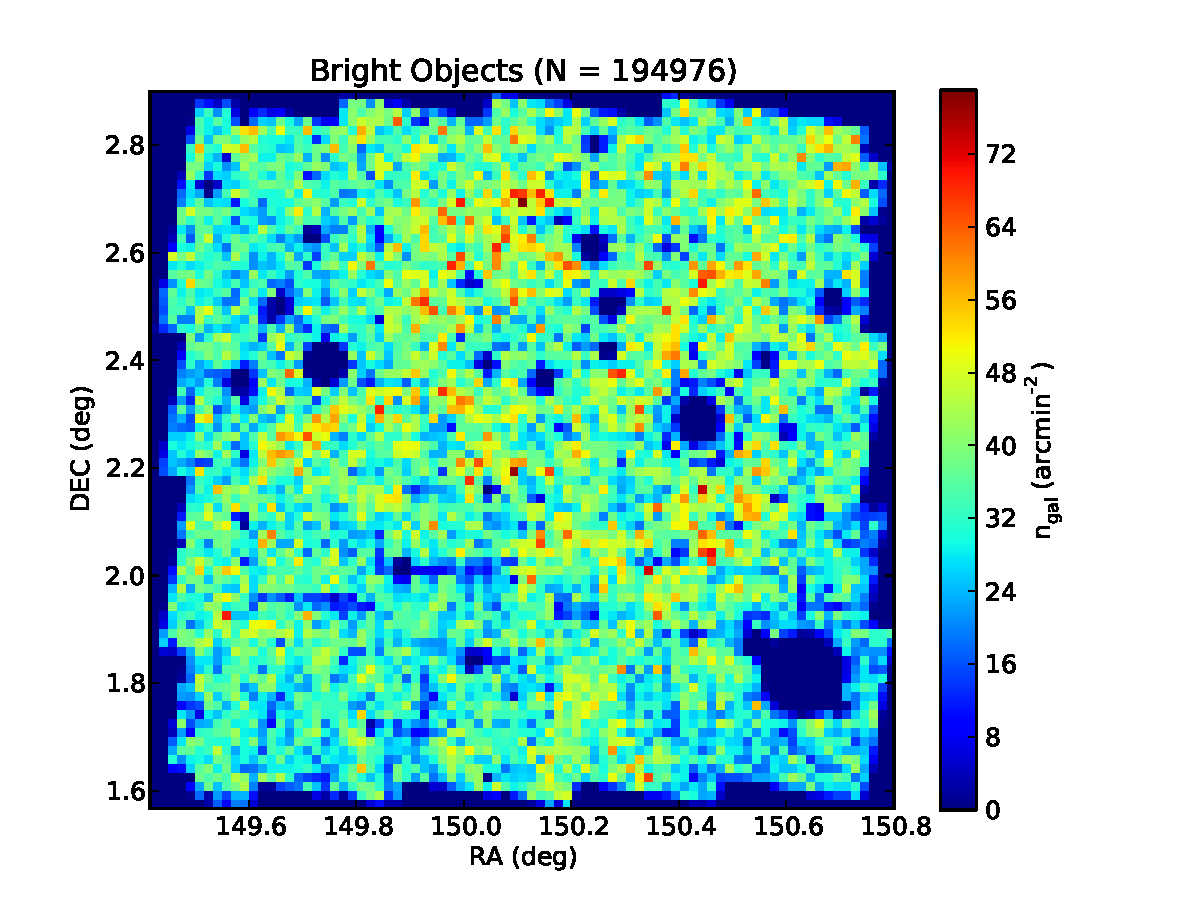
\includegraphics[width=0.8\textwidth]{locations_bright.pdf}
  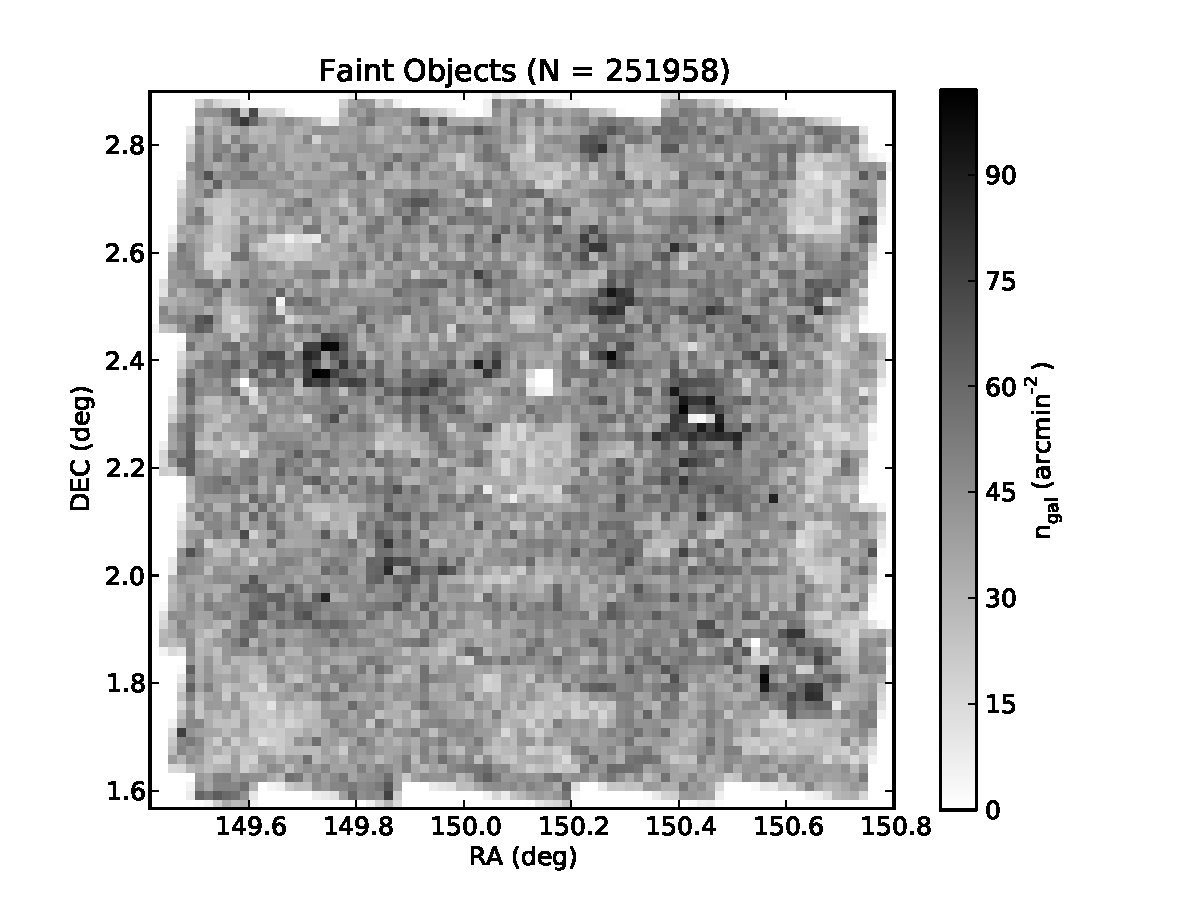
\includegraphics[width=0.8\textwidth]{locations_faint.pdf}
  \caption{Angular locations of the 194,976 COSMOS galaxies with photometric
    redshift measurements (top panel)
    and the 251,958 COSMOS galaxies without photometric redshift estimates
    (bottom panel).}
  \label{fig:COSMOS_locations}
\end{figure}

\begin{figure}
  \centering
  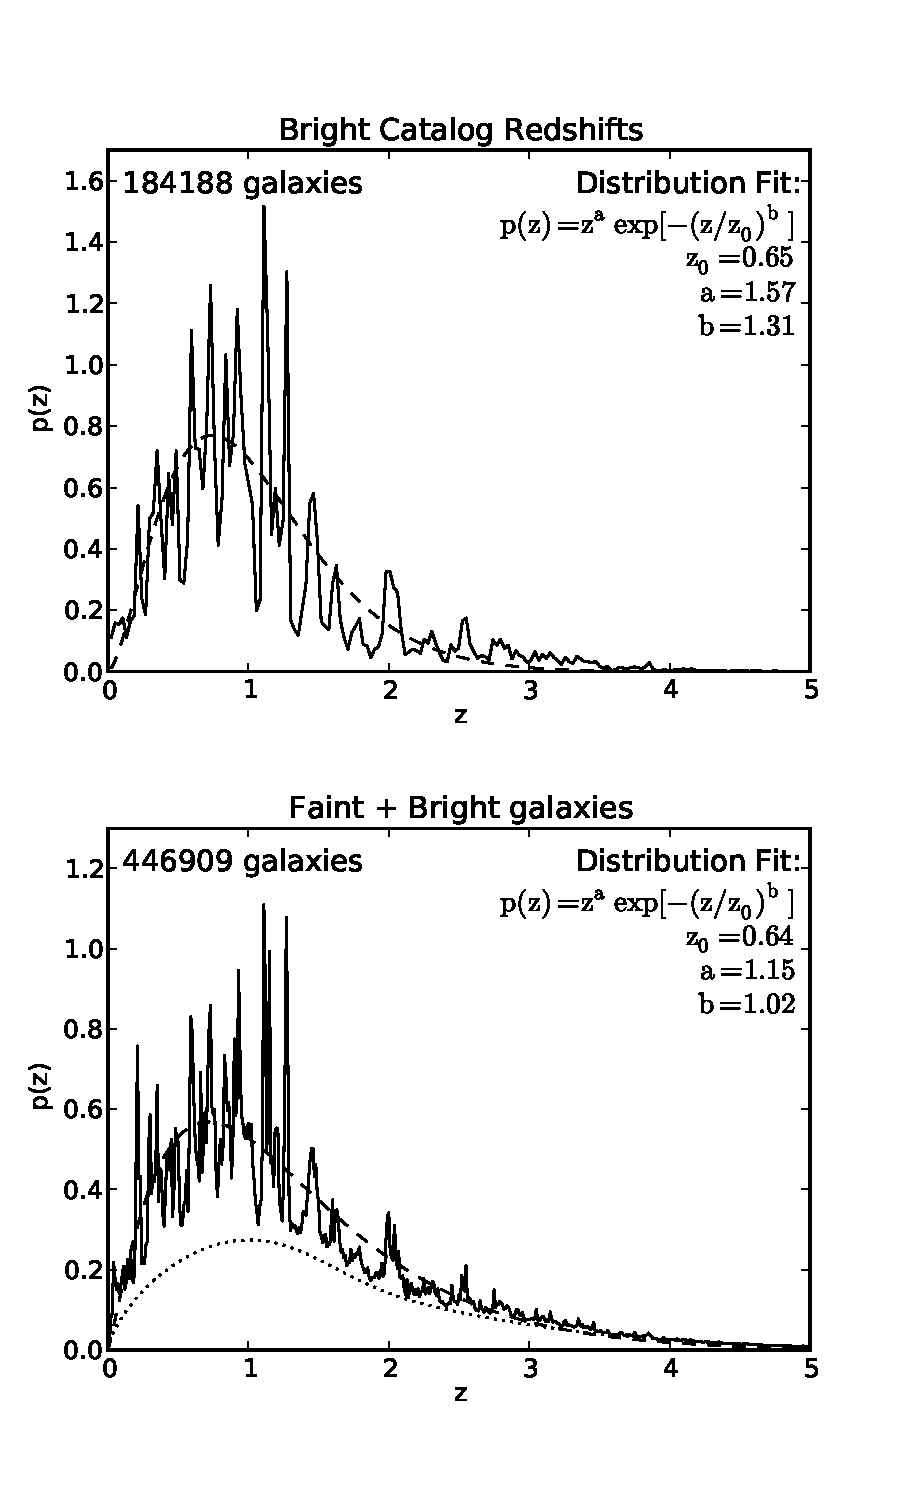
\includegraphics[width=0.8\textwidth]{zdist.pdf}
  \caption{Redshift distributions of the COSMOS data.  The top panel shows the
    distribution of photometric redshifts of the shear catalog cross-matched
    with the COSMOS30 photometric redshift catalog \citep{Ilbert09}, while
    the bottom panel includes the inferred redshift distribution of the
    remaining faint galaxies.}
  \label{fig:COSMOS_zdist}
\end{figure}

In addition, S10 identifies potential catastrophic outliers in the redshifts.
Photometric redshifts gain significant leverage from broad spectral features
such as the Lyman and Balmer spectral breaks.  The Balmer limit is
$\sim 364$nm, while the Lyman limit is $\sim 91$nm, so that the Balmer limit
of a galaxy at redshift $z_0$ is at the same observed wavelength as the
Lyman limit at redshift $z_0 + 3$.  This can lead to a degeneracy in redshift
determination that results in catastrophic outliers -- that is, low redshift
galaxies identified as high redshift, or high redshift galaxies identified as
low redshift.  In shear studies, the former acts to dilute the high-$z$
shear signal,
while the latter acts to add spurious signal at low redshift.  To prevent
the latter effect from affecting results, we follow S10 and remove galaxies
with $i^+ > 24$ and redshifts $z < 0.6$.  S10 provides several tests which
show that this cut does not generate appreciable systematic error.

S10 performs a classical shear correlation function analysis to find
constraints on $\sigma_8$ and $\Omega_M$ which are consistent with
those derived from WMAP: for a flat $\Lambda$CDM cosmology, they
find with 63\% confidence 
$\sigma_8(\Omega_M / 0.3)^{0.51} = 0.79 \pm 0.09$.  S10 performs both a
two-dimensional analysis and a three dimensional analysis: the constraints
from each are consistent, with a slightly better figure of merit for the
$\Omega_M$ vs. $\sigma_8$ constraint when the analysis is computed within
several redshift bins.  The strength of the
3D treatment comes when the assumption of flatness and/or equation of
state for dark energy is dropped: for a
$\Lambda$CDM cosmology with varying dark energy equation of state $w$,
they find at 90\% confidence that $w < -0.41$.
Though these constraints offer only a slight improvement over prior
information from WMAP constraints from measurements of the CMB, we must
note that they are derived from just over
1 square degree of observations, while the
WMAP constraints use the full sky.  Future wide-field
lensing surveys will be able to place much more competetive constraints
on these parameters.

Here we will not duplicate all the various analyses of S10: instead we
will use the KL-based estimation formalism of \S\ref{sec:KL_bayes} with
shear eigenbases computed for the observed field via the formalism
of \S\ref{sec:KL_shear}.  This will allow us to constrain two-point
information using the KL formalism.

\subsection{Intrinsic Ellipticity estimation}
\label{sec:bootstrap}
In order to apply the KL analysis techniques discussed
above and in Chapter 2, we require an accurate
determination of the noise for the observed shear.  Assuming systematic
errors are negligible, shape noise should be dominated by shot noise,
which scales as $\mymat{\mathcal{N}}_{ii} = \hat{\sigma}_\epsilon^2 / n_i$,
with $n_i$ representing the number of galaxies in bin $i$.

To test this assumption, we perform a bootstrap resampling of the observed
shear in square pixels which are two arcminutes on a side.
Generating 1000 bootstrap samples within each
pixel, we compute the variance in each pixel.
From Poisson statistics, we would expect the variance in each pixel to
scale inversely with the number of measurements within each pixel: with this
in mind we plot in Fiugre~\ref{fig:bootstrap}
the variance vs the number of galaxies and fit a curve of the form 
\begin{equation}
  \sigma_\gamma^2 = \frac{\sigma_{int}^2}{n_{\rm gal}},
\end{equation}
where $\sigma_{int}$ is the intrinsic ellipticity dispersion of the population.
As shown in the upper panel of Figure~\ref{fig:bootstrap}, the best-fit
curve has $\sigma_{int} = 0.393$.  The residual distribution, shown in the
lower panel of the figure, is close to Gaussian as expected.

In this figure, we see that the fluctuation in shape noise from pixel to
pixel is only a few percent.  For the analysis below, we use for each pixel
the bootstrapped estimates derived here.  Because bootstrapping is inaccurate
for pixels with a small number of galaxies, if a pixel has fewer than 10
sources we use the best-fit estimate for the noise,
$\mymat{\mathcal{N}}_{ii} = \hat{\sigma}_\epsilon^2 / n_i$
with $\hat{\sigma}_\epsilon = 0.392$.  Pixels with zero galaxies (i.e.
masked pixels) are treated using the techniques developed in
Section~\ref{sec:kl_intro}.

\begin{figure*}
 \centering
 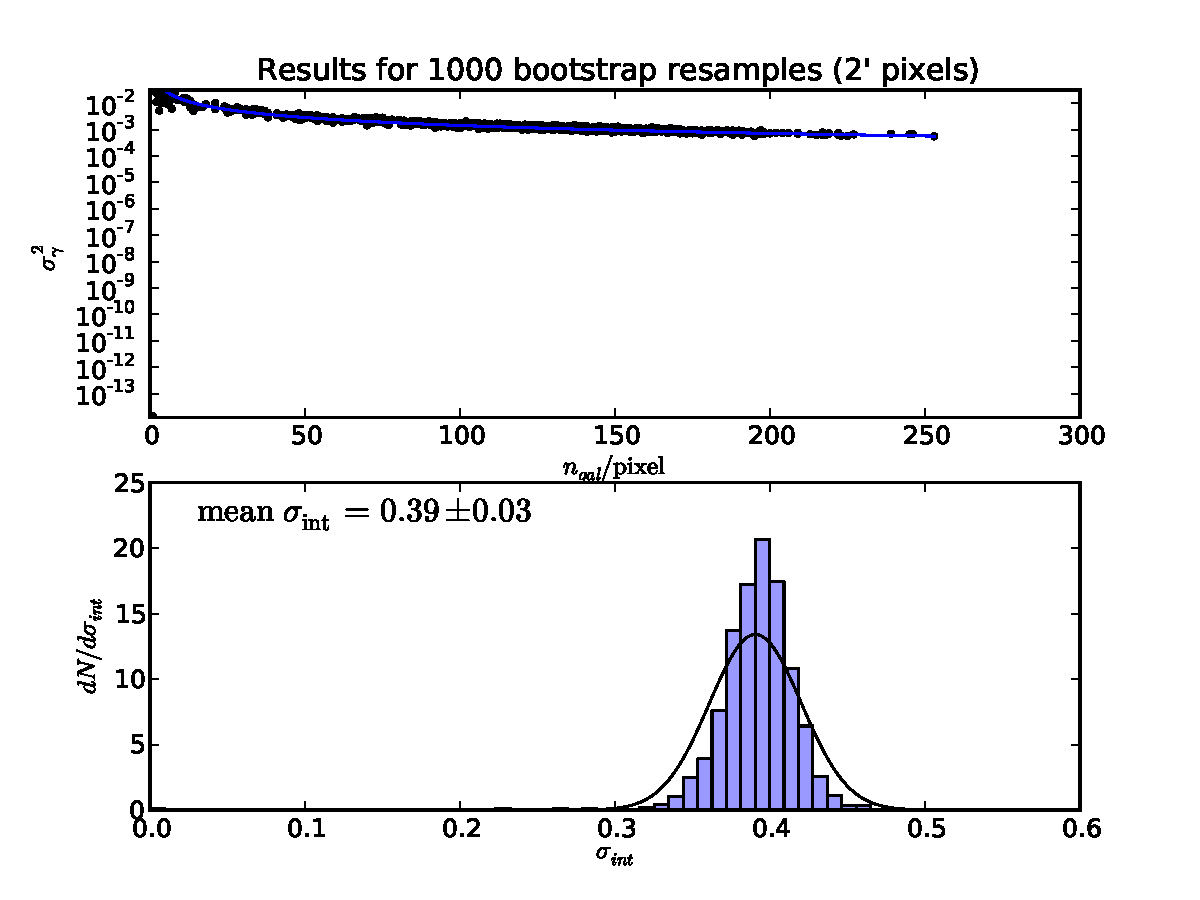
\includegraphics[width=0.8\textwidth]{sigma_calc.pdf}
 \caption{Bootstrap estimates of the shape noise for each pixel.  The estimates
   reflect an intrinsic ellipticity of $0.393 \pm 0.013$.
   \label{fig:bootstrap}}
\end{figure*}

\subsection{Whitened KL modes}
Using the pixel-by-pixel noise estimates from the previous section, we can
now follow the formalism of \S\ref{sec:kl_intro} and construct the optimal
orthonormal basis across the survey window defined by the selection function
of the bright galaxies from the COSMOS survey.  We use pixels which are
two arcminutes on a side, in a grid of 40 $\times$ 41 = 1640 total
pixels.  We whiten the theoretical correlation matrix according to the noise
properties of the observed data, and compute the eigenvalue decomposition
of the resulting correlation matrix.

The first nine eigenmodes for the bright galaxy sample
are shown in Figure~\ref{fig:eigenmodes}.
It is interesting to compare these to the modes shown in
Figure~\ref{fig_KL_modes}, which are derived under the assumption that
each pixel has the same number of sources, and thus the same noise properties.
The window function of the COSMOS survey is clearly present, as can be
seen by comparing the
masking apparent in the eigenmodes to that of the galaxy distribution
shown in the upper panel of Figure~\ref{fig:COSMOS_locations}.
Moreover, the asymmetry of the mask acts as a perturbation which destroys
the rotational symmetry evident in the idealized eigenmodes of
the previous chapter.

\begin{figure*}
 \centering
 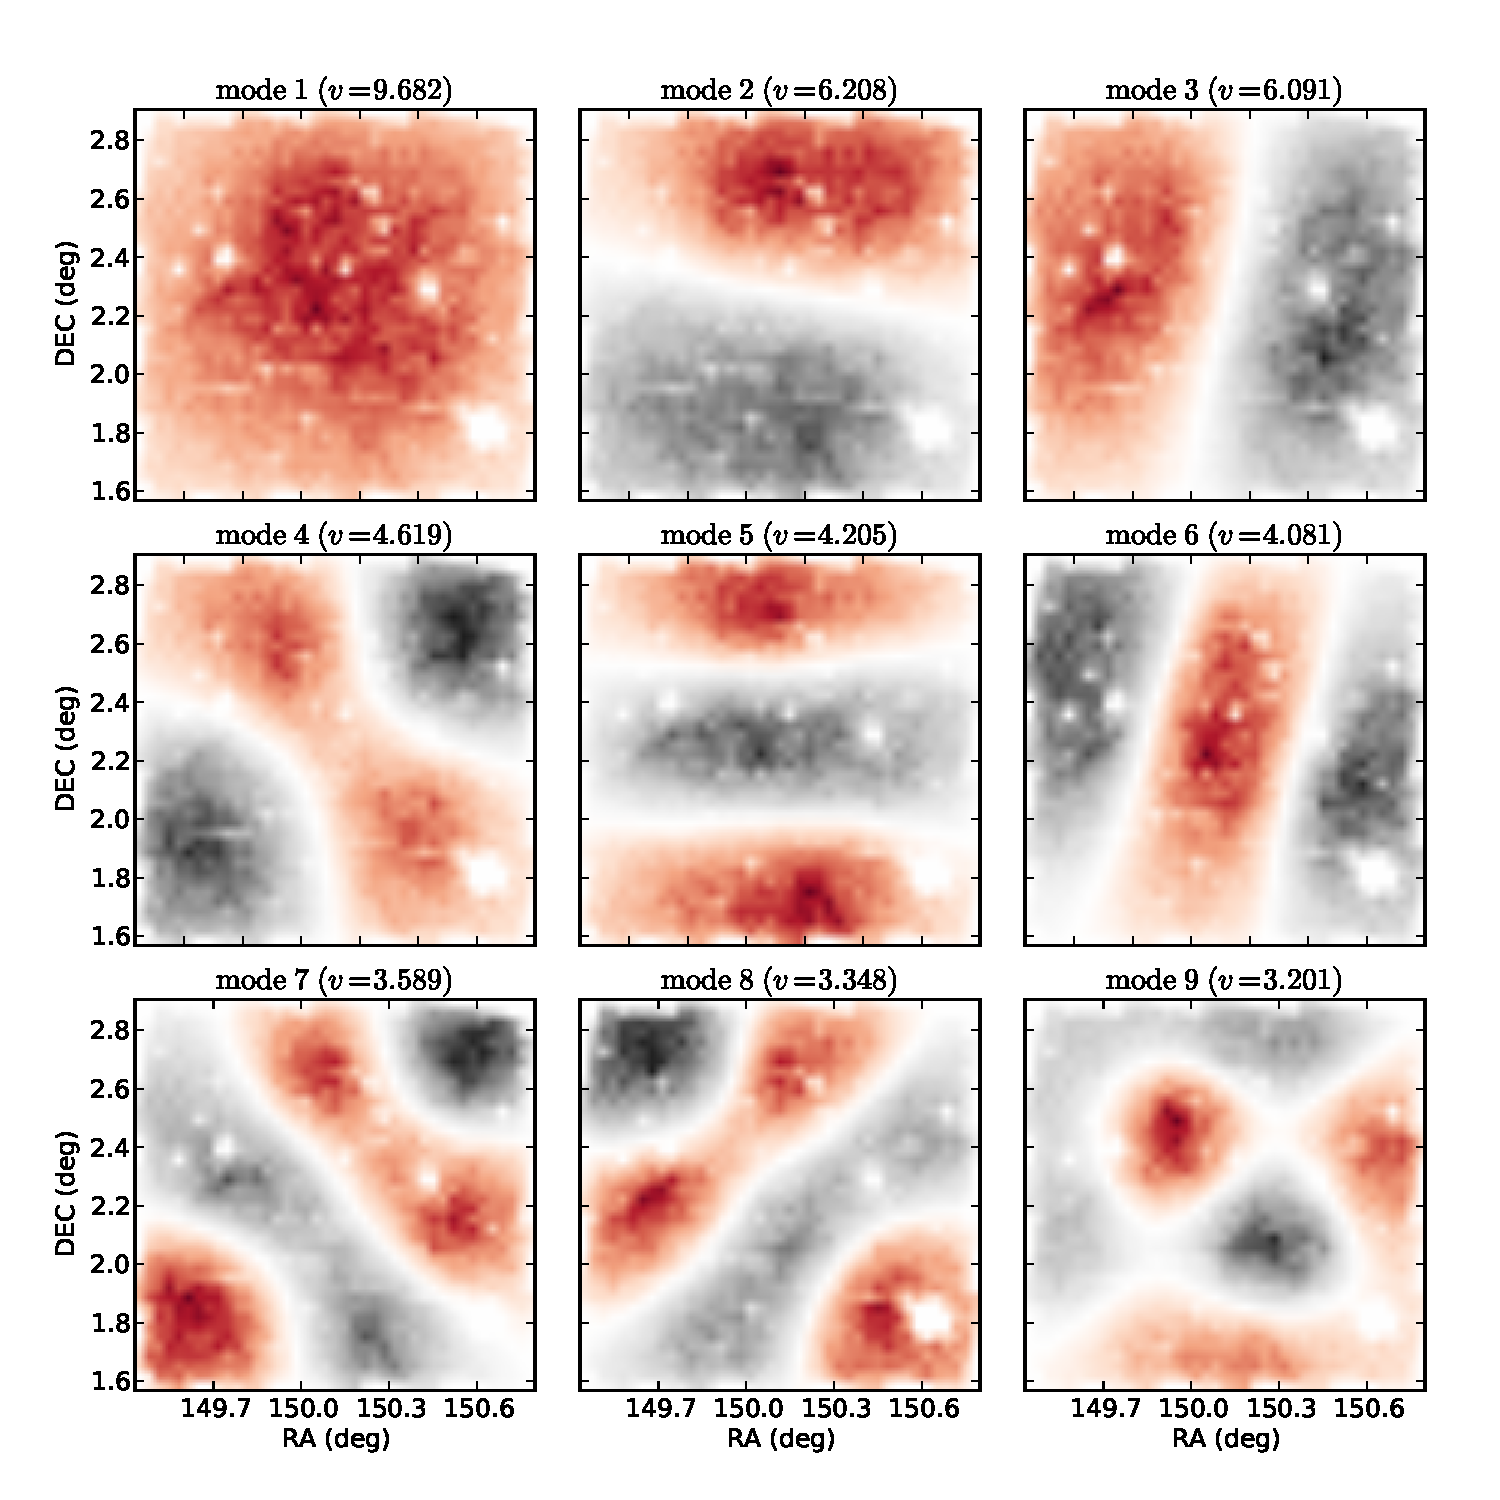
\includegraphics[width=\textwidth]{bright_eigenmodes.pdf}
 \caption{
   The first nine 2D KL signal-to-noise eigenmodes
   for the COSMOS bright objects.  This uses square pixels which are
   two arcminutes on a side, leading to $41 \times 40 = 1640$ pixels
   over the entire field.}
   \label{fig:eigenmodes}
\end{figure*}

The eigenvalues of the whitened correlation matrix are shown in
Figure~\ref{fig:eigenvalues}.  Because the covariance matrix is
whitened, the noise is normalized to $1$ within each mode.
Similar to the results seen in the previous chapter, only a very small
number of modes have signal-to-noise greater than 1.
This figure also shows that the signal drops to zero at just over 1500
modes.  This is due to the survey mask: approximately 120 of the 1640
modes are completely masked, such that they have no signal and do not
contribute to the correlation matrix.

As discussed above, an advantage of KL is its ability to yield an optimal
low-rank approximation of a set of observations, by truncating the low
signal-to-noise modes in a reconstruction.  The choice of which modes to
truncate for a reconstruction or other analysis is not straightforward:
as discussed in Chapters 3-4, this decision amounts to a tradeoff between
systematic bias and statistical error.  Below we impose a cutoff for
modes with signal-to-noise ratios of less than $\sim 1/10$, corresponding to
mode number 800.  This lies approximately at the inflection point of the
signal-to-noise curve.

\begin{figure*}
 \centering
 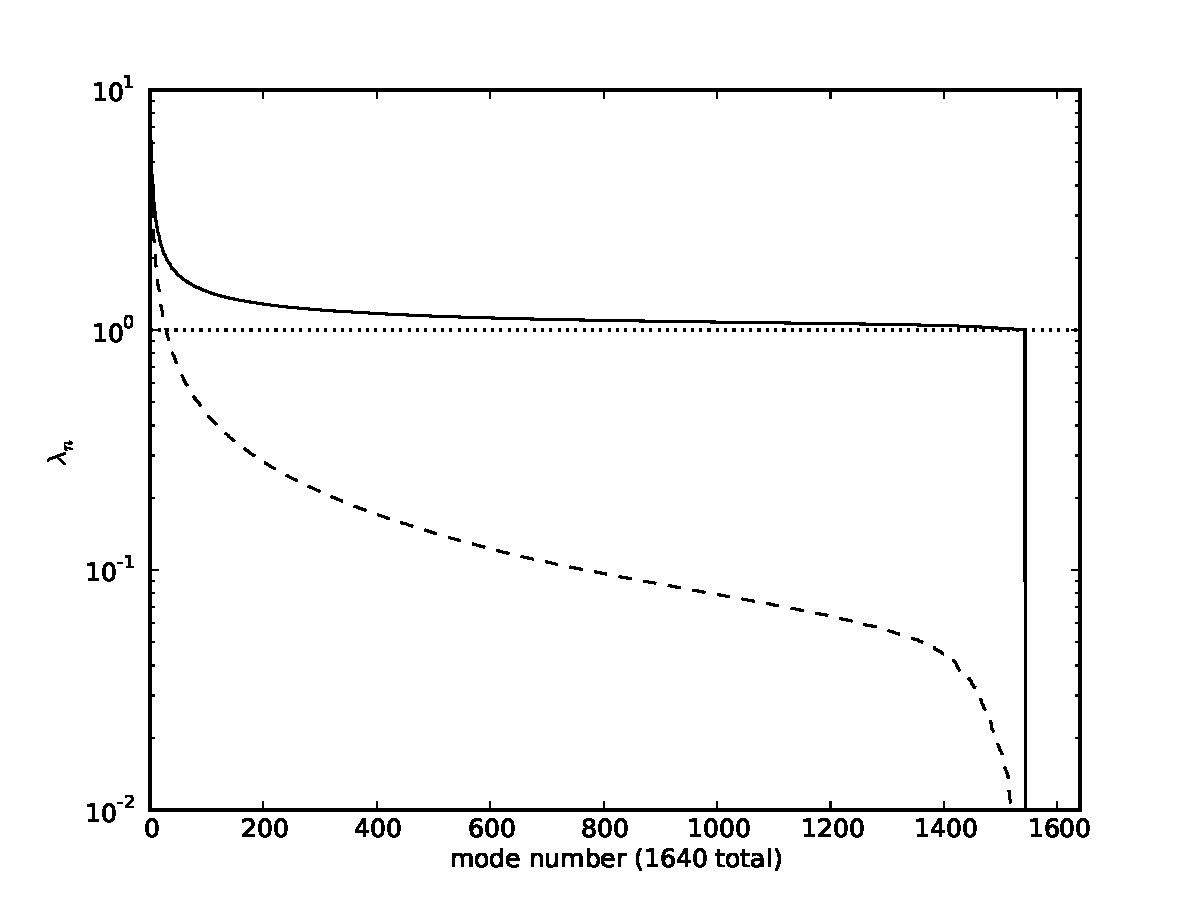
\includegraphics[width=0.8\textwidth]{bright_eigenvalues.pdf}
 \caption{
   The distribution of KL eigenvalues for the eigenmodes shown
   in Figure~\ref{fig:eigenmodes}.  There are $41 \times 40 = 1640$
   pixels, but approximately 90 of these contain no sources and are part of
   the mask.  This is reflected in the fact that the final 90 KL modes have
   zero eigenvalue.}
   \label{fig:eigenvalues}
\end{figure*}

\subsection{Is our shear Gaussian?}
The KL formalism for shear analysis assumes that the shear is well-described
by a Gaussian random field described by a covariance matrix, with mean
zero.  If this is the case, then (by the arguments of chapter 2) we would
expect the observed KL coefficients of the whitened signal to be Gaussian
distributed with zero mean and variance equal to the associated eigenvalue.
Figure~\ref{fig:coeff_hist} shows a histogram of the observed coefficients
scaled by the corresponding eigenvalue.  As is evident, both the real
part and the imaginary part of the scaled coefficients are consistent with
being drawn from a standard normal distribution.  This is consistent with
our assumption that the shear is drawn from a gaussian random field, and
that the noise properties estimated in \S\ref{sec:bootstrap} are accurate.

\begin{figure*}
 \centering
 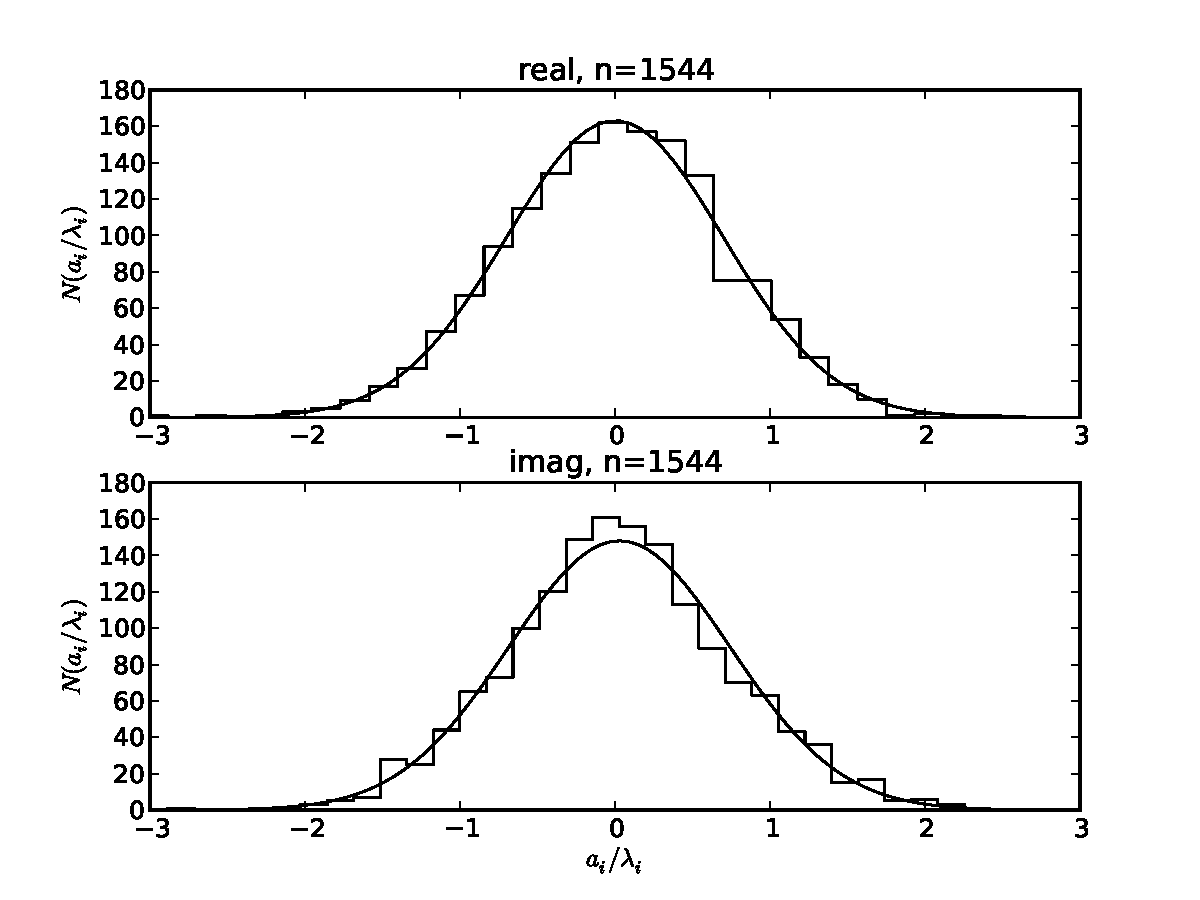
\includegraphics[width=0.8\textwidth]{bright_coeff_hist.pdf}
 \caption{
   The histogram of normalized coefficients $a_i / \sqrt{\lambda_i}$.
   If the shear is truly a gaussian random field, this distribution should
   be a gaussian with unit variance.
   \label{fig:coeff_hist}}
\end{figure*}

\subsection{Relationship to Power Spectrum}
As we did in Figure~\ref{fig_bandpower}, for each KL mode we can compute the
associated two-dimensional power spectrum to determine the relationship
between each mode and the Fourier power it represents.  For the unmasked
KL modes explored in the previous chapter, this relationship displayed a
fairly tight scatter between KL mode number and Fourier mode number.
As seen in Figure~\ref{fig:bandpower_masked}, however, we see that the
masked KL modes have a much larger scatter in associated Fourier modes,
especially for higher KL mode numbers.

The analysis reflected in this plot can help in the choice of which KL
modes to truncate: the pixel scale is two arcmin, which corresponds to
$\ell = (2\pi\ {\rm rad}) / (2\ {\rm arcmin}) \approx 10000$.  So modes
which do not have significant Fourier power on angular scales
$\ell < 10,000$ are likely to be limited in their usefulness for parameter
estimation from the gridded shear.

\begin{figure*}
 \centering
 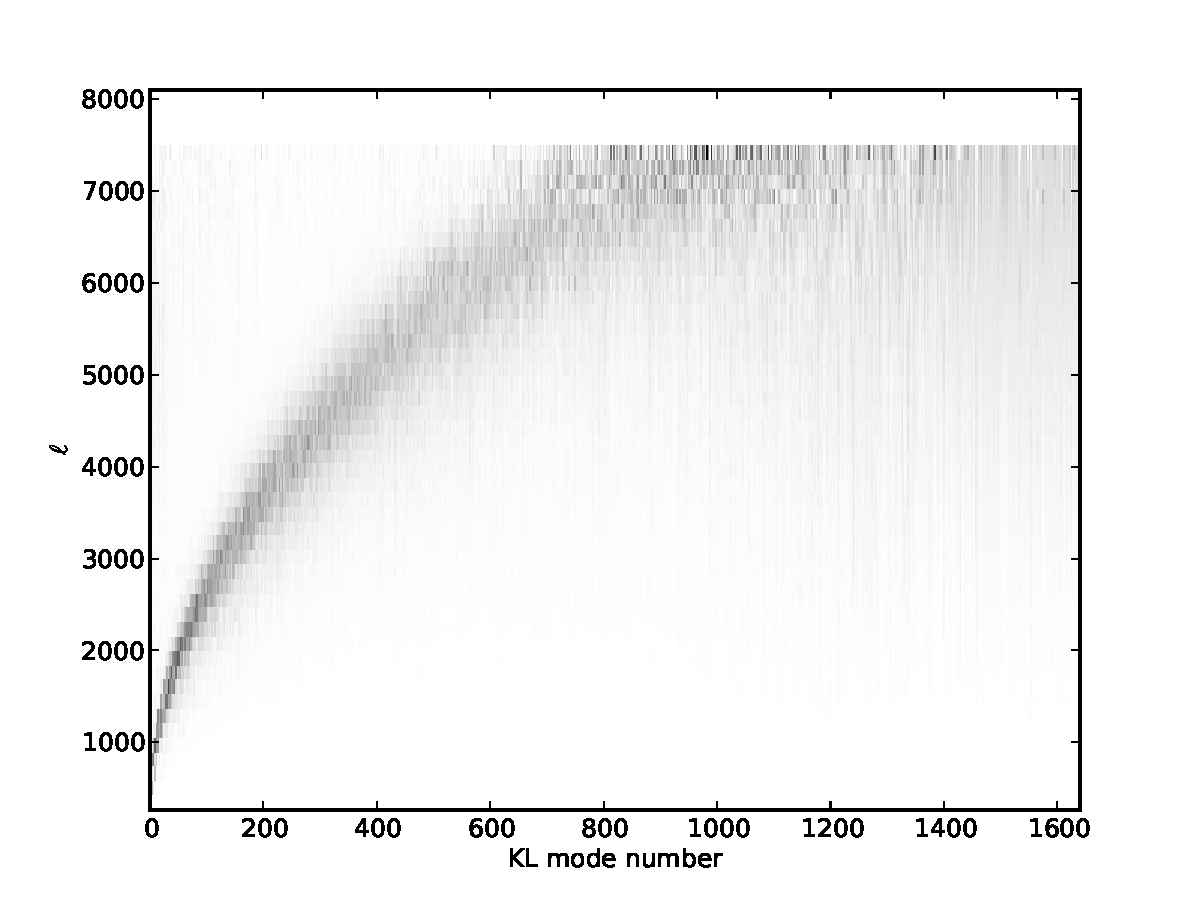
\includegraphics[width=0.8\textwidth]{bright_bandpower.pdf}
 \caption{
   The fourier power represented by each KL mode.  For each KL mode number,
   the vertical band shows the distribution of power with angular wavenumber
   $\ell$.  In general, the larger KL modes correspond to larger values of
   $\ell$, though there is a lot of mode mixing.
   \label{fig:bandpower_masked}}
\end{figure*}

\section{Results}
\label{sec:results}
The result of the KL-based Bayesian inference for cosmological parameter
estimation is shown in Figure~\ref{fig:posterior}.  To compute the
eigenmodes, we assume a flat $\Lambda$CDM cosmology with
$\Omega_M = 0.27$, $\Omega_L = 0.73$, $\sigma_8 = 0.812$, and $h=0.71$.
These KL modes are computed for the angular and redshift distribution
of the bright galaxy sample, and the KL-based Bayesian inference is
performed assuming flat cosmology.  We use only a single redshift bin in
this case, which is comparable to the first analysis performed in
S10.

The 
This leads to a best-fit cosmology $\Omega_M = 0.23 \pm 0.06$,
$\sigma_8 = 0.83 \pm 0.09$, where the error bars represent 1$\sigma$
deviations at maximum.
This does not capture the entire story, however, as there
is a strong degeneracy between the parameters (note that WMAP data offers
complementary constraints in this plane, and can be used to break this
degeneracy: see S10).  Following S10, we describe this degeneracy by
computing a power-law fit to the posterior distribution, to find
\begin{equation}
  \sigma_8 (\Omega_M / 0.3) ^ {1.03} = 0.88 \pm 0.14.
\end{equation}
This should be compared to the S10 result for the 2D analysis,
$\sigma_8 (\Omega_M / 0.3) ^ {0.62} = 0.62 \pm 0.11$.

Compared to S10, our results show a 50\% broader constraint on $\sigma_8$,
as well as a stronger degeneracy between $\sigma_8$ and $\Omega_M$ 
(reflected in the exponent of the relation).  This discrepancy is likely
due to the fact that we use only the bright galaxies in this analysis,
while the S10 results use both bright and faint galaxies, as well as the
fact that S10 marginalizes over nuisance parameters (the hubble parameter
and redshift systematic corrections) while we fix these at the  expected
values.

S10 notes that the low value of $\sigma_8$ seen in their 2D analysis is likely
an artifact of cosmic variance: the strongest contributions to lensing
signals in COSMOS are from z > 0.7, which boosts the shear signal for higher
redshift sources but leads to a lower signal at intermediate reshifts.
Using the full 3D analysis, S10 is able to separate these regions, leading
to results consistent with those from WMAP.

Here we have limited the analysis to two dimesnions, but this is by no means a
fundamental limitation of KL.  As long as we can sufficiently estimate the
correlation of signal and noise, KL can be used to analyze an arbitrary
geometry: in future work we will extend the present analysis to three
dimensions, fully taking into account the redshifts of the sources.

\begin{figure*}
 \centering
 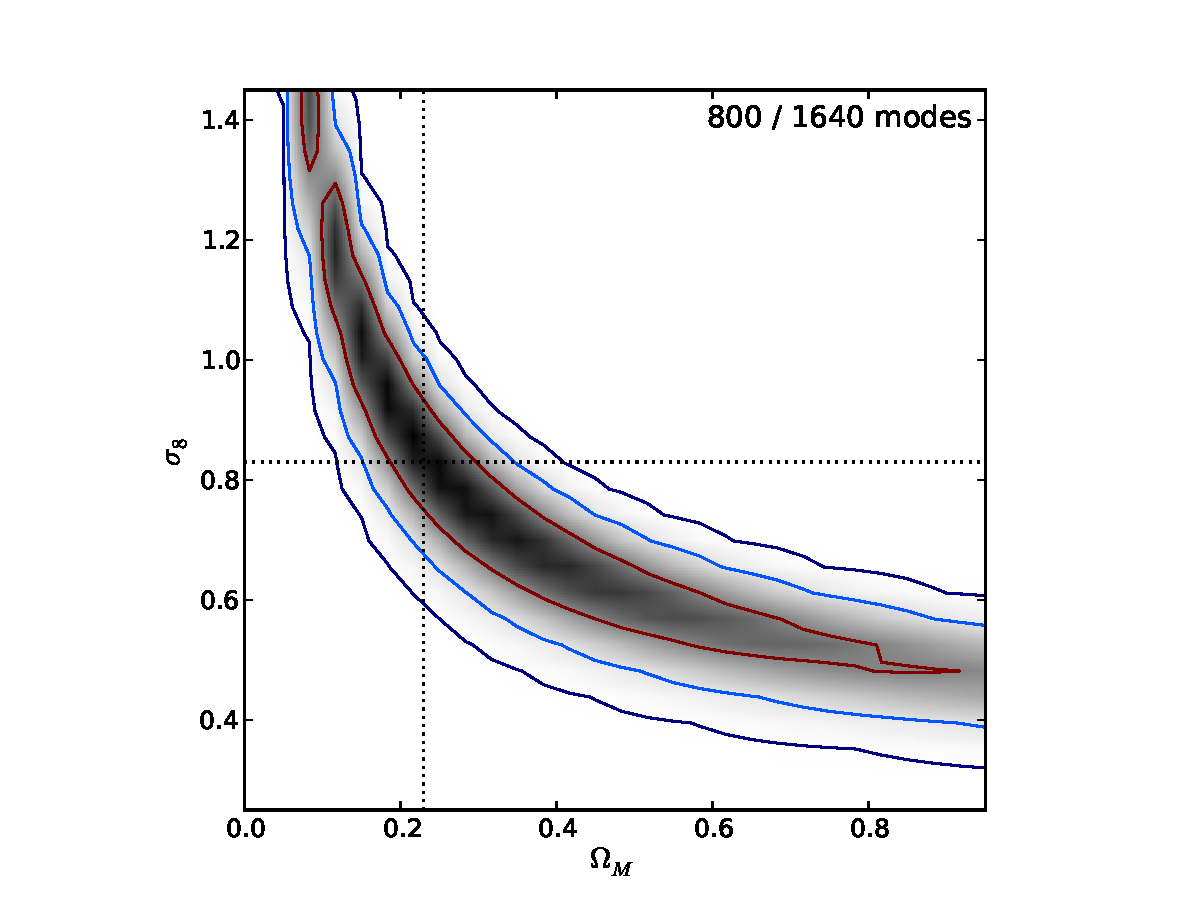
\includegraphics[width=0.8\textwidth]{posterior.pdf}
 \caption{The posterior distribution in the $(\Omega_M, \sigma_8)$ plane
   for a 2D analysis of the bright galaxy sample.  This uses 800 of the
   1640 modes, such that the truncated modes have average signal-to-noise
   ratios of $<\sim 1/10$, and an approximate angular scale of
   $\ell \sim 7000$, which corresponds to 3 arcmin or 1.5 pixel-lengths.}
 \label{fig:posterior}
\end{figure*}

